% !TEX encoding = UTF-8 Unicode
% !TEX root = project.tex

\section{Introduction}
\label{sec:intro}
According to Gartner, global software expenditures for 2015 amounted to \$3.52 trillion, and forcasted to grow 0.6 \% to \$3.54 trillion in 2016\cite{gartner2016}.\\

In any large scale project, as the teams and team size increases, size of the source code repositories as well as the number of lines of code (LOC) increase slowly. As the repositories increase in size, dependencies amongst all the objects in the repository also increases. After a certain point of time, it becomes extremely difficult for developers and managers to track these repositories. \\

From developer's perspective, to make any changes to the code, they will have to look deep inside the repository to see effects of their changes. Many simple tools provide that service in a very orthodox way (plain text format). For example, in Eclipse, on using Open Call Hierarchy for a method, it gives a list of all the other methods from various classes that are calling this method. In small projects, this can be helpful but in large size projects, finding relevant method becomes a tedious task. \\

From manager's perspective, they need to understand the design and architecture of the project, and defect-prone critical areas in it, so that resource allocation can be easily done in a optimized way. Managers usually have strong domain knowledge but at times, they lack technical design and architectural knowledge. So, if they have to make any critical decisions (like resource allocation), lack of sufficient knowledge on product/software specific information might lead to bad results (under/over allocation of resources).\\

So, to help developers and managers, we implemented Noodlr, a web based tool which can be used with any source code repository to get a detailed view. Developers can use it to check the dependencies and relationships between various programming components (like classes, methods and packages). So, before a developer makes any change in the code with respect to a defect resolution, he/she can use this tool to check the side-effects on other objects, if any. Managers can use this tool to detect the most defect-prone areas and hence can do resource allocation appropriately. \\

Also, in large projects, teams focusing on different areas work together with lots of dependencies between them. Many a times, work allocation becomes a problem for managers as they are not sure as to which team a particular piece of work should be assigned. This tool can be used to create the module boundaries as well, which makes the manager's job of work allocation easier.\\

Noodlr is an interactive web based tool, implemented in D3.js with a Java-based backend, that constructs a dependency graph for a given repository and shows all the parent-child relations, static call-dependencies and strongly connected components (using Kosaraju-Sharir's algorithm\cite{sharir1981strong}). In this project, we have attempted to achieve the following objectives:
\begin{enumerate}
    \item Implement a web based tool which provides an interactive graphical user interface (GUI) to explore the whole source code repository.
    \item Finding areas in the source code repository where the probability of getting defects is high. We have used Kosaraju-Sharir algorithm and Bron-Kerbosch algorithm for this purpose.
    \item Evaluate the efficiency of Kosaraju-Sharir algorithm and Bron-Kerbosch algorithm on few well-known open source projects.
    \item Evaluate if Noodlr gives appropriate results using the above mentioned algorithms by comparing it to the files in Github pull requests that are related to issues.
\end{enumerate}

In section \ref{sec:algos}, we discuss two major algorithms that we have used in our tool to find the defect-prone areas. In section \ref{sec:related}, we provide the motivation behind our project by explaining some of the related works. Thereafter, we discuss the software implementation of Noodlr in section \ref{sec:setup} as well as the backend server that implements Kosaraju-Sharir and Bron-Kerbosch algorithm. In the evaluation covered in section \ref{sec:finding}, we present the experimental study that was conducted on open source github repositories. For our study, we used a medium sized repository called Retrofit (around 9000 LOC) from Square Inc, a large sized repository called Twitter4j (around 33000 LOC) maintained by an independent developer, a third repository named Guava (around 143000 LOC) from Google and a small repository named Scribejava (around 5000 LOC). The last 2 repositories were not used for our visualization purposes and were used only for evaluation. In section \ref{sec:threats}, we discuss few short comings of our tool that we found from our evaluation and also discuss few drawbacks of one of the algorithms. In section \ref{sec:practical}, we discuss some of the practical applications of our tool. In section \ref{sec:conclusion}, we discuss the future work related to our tool and finally conclude the paper.

\section{Terminologies and Algorithms}
\label{sec:algos}

We attempt to use a couple of graph algorithms for the purpose of detecting defect-prone areas in a software project. First we construct graphs from the class dependencies and the method dependencies in the project. To restrict the scope of our work, we concentrate only on projects that use Java\footnote{\url{https://www.oracle.com/java/index.html}} as the main programming language. The graph is constructed with classes or methods forming the vertexes of the graph and the relationship between classes or methods forming the edges between the vertexes. Once the graph is fully constructed, we try to find the strongly connected components (SCC) using Kosaraju's algorithm (a.k.a Kosaraju-Sharir algorithm). We also try to find out maximal cliques using Bron-Kerbosch algorithm. 

\subsection{Strongly connected components (SCC)}
In the mathematical theory of directed graphs, a graph is said to be strongly connected if every vertex is reachable from every other vertex. The strongly connected components of an arbitrary directed graph form a partition into subgraphs that are themselves strongly connected\footnote{\url{https://en.wikipedia.org/wiki/Strongly_connected_component}}. Figure~\ref{fig:scc_sample} shows a sample graph marked with strongly connected components.

\begin{figure}[h!]
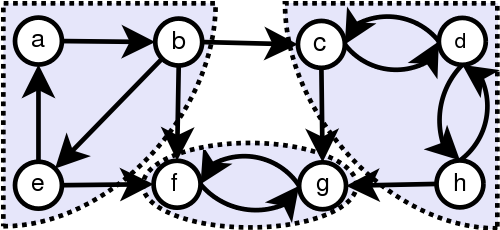
\includegraphics[width=8cm]{scc_sample}
\caption{SCC's marked in a sample graph}
\label{fig:scc_sample}
\end{figure}

\subsection{Kosaraju-Sharir algorithm}
Kosaraju-Sharir algorithm\cite{sharir1981strong} is a linear time algorithm to find the strongly connected components of a directed graph. Kosaraju's algorithm uses two passes of depth first search. The first pass is used to choose the order in which the outer loop of the second depth first search checks vertices for having been visited already and recursively explores them if not visited already. The second depth first search is on the transposed graph of the original graph, and each recursive exploration finds a new strongly connected component\cite{cormen2001introduction}.

\subsection{Maximal cliques}
A clique is a set of nodes in a graph where between every pair of nodes (X, Y) a dependency exists. A clique is maximal if no other node can be added without losing the clique property\cite{zimmermann2008predicting}. We attempt to find out maximal cliques from the graph constructed earlier and check whether it can be used for predicting the defect-prone areas of the project. To find the maximal cliques, we assume that the nodes in the graph is undirected. i.e., even though there is a direction in the dependency of classes or methods, for the purpose of finding maximal cliques, we let go of the direction of dependency.

\subsection{Bron-Kerbosch algorithm}
Bron-Kerbosch algorithm\cite{bron1973algorithm} is used to find maximal cliques in an undirected graph. We used the version of the algorithm which does not have pivoting. Although this algorithm is used in previous studies\cite{zimmermann2008predicting} to predict defect-prone areas, we were unsuccessful in our attempt to get any result by applying this algorithm on the software projects we selected. We conjecture that this may be due to the particular structure of the projects that we selected that did not have a maximal clique present in their structure.

